% This here was due to a save stack issue with global assignments of
% pgfstrokecolor and pgffillcolor. 
%
% It does not really fit into this regression framework; but I wanted
% to keep the test (but I suppose it needs to be executed manually)

\documentclass{article}

\usepackage{tikz}
\usepgflibrary{arrows.meta}

\begin{document}

\begin{tikzpicture}
	\begingroup
		{
		\pgfsetstrokecolor{green}
		}
		\pgfscope
		\draw[-stealth] (0,1) -- (1,1);
		\endpgfscope
	\endgroup

\end{tikzpicture}

\begin{tikzpicture}
	\begingroup
		\pgfscope
		\pgfsetstrokecolor{green}
		\pgfscope
		\pgfsetstrokecolor{red}
		\draw[-stealth] (0,1) -- (1,1);
		\endpgfscope
		\draw[-stealth] (1,1) -- (2,1);
		\endpgfscope
	\endgroup

\end{tikzpicture}


\tikz [ultra thick] \draw [blue, arrows = {-stealth}] (0,0) -- (1,0);

\tikz [ultra thick] \draw [red, arrows = {-stealth[color=blue]}] (0,0) -- (1,0);

\tikz [ultra thick] \draw [draw=red, fill=red!50, arrows = {-stealth[length=10pt]}]
                          (0,0) -- (1,1) -- (2,0);

\tikz {
  \draw [help lines] (0,-.5) grid [step=1mm] (1,.5);
  \draw [thick, red, arrows = {-Stealth[fill=white,length=15pt]}] (0,0) -- (1,0);
}

\tikz {
  \draw [help lines] (0,-.5) grid [step=1mm] (1,.5);
  \draw [thick, red, arrows = {-Stealth[fill=none,length=15pt]}] (0,0) -- (1,0);
}

\tikz {
  \draw [help lines] (0,-.5) grid [step=1mm] (1,.5);
  \draw [thick, red, arrows = {-Stealth[color=blue, fill=white, length=15pt]}]
        (0,0) -- (1,0);
}

\tikz [ultra thick] \draw [draw=red, fill=red!50,
                           arrows = {-Stealth[length=15pt, fill=pgffillcolor]}]
                          (0,0) -- (1,1) -- (2,0);

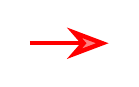
\begin{tikzpicture}
%\tracingcommands=2\tracingmacros=2
	\begingroup
		{
		\pgfsetfillcolor{red!50}
		}
		\pgfscope
		\draw[ultra thick,draw=red,arrows={-Stealth[length=15pt, fill=pgffillcolor]}] (0,1) -- (1,1);
		\endpgfscope
	\endgroup

\end{tikzpicture}

\tikz [ultra thick] \draw [double,blue, arrows = {-stealth}] (0,0) -- (1,0);
\end{document}

